\section{Theory}
The Geiger-M{\"u}ller (GM) counter is a radiation detection device used to measure ionizing radiation, such as alpha, beta, and gamma rays. It operates by detecting the ionization produced by radiation in a gas-filled tube, leading to an electrical pulse that is counted and displayed. GM counters are widely used in radiation safety monitoring, environmental surveys, nuclear industry applications, medical radiation detection, and laboratory research. Their high sensitivity to radiation and ease of use make them valuable tools for detecting and measuring radiation levels in various settings.

The Geiger-Muller (GM) counter works by detecting the ion-electron pairs created by the interaction of charged particles in a gas mixture. The GM tube is a metal cylinder with a thin wire (anode) at its axis and a metal cylinder (cathode) maintained at a high voltage to create an electric field. The radiation enters through a window on the tube, creating ion-electron pairs that are swept by the electric field to produce a phenomenon called an avalanche, which generates output pulses that are counted by related circuits. A schematic diagram of the GM counter is shown in Fig. \ref{t1}.

\begin{figure}
    \centering
    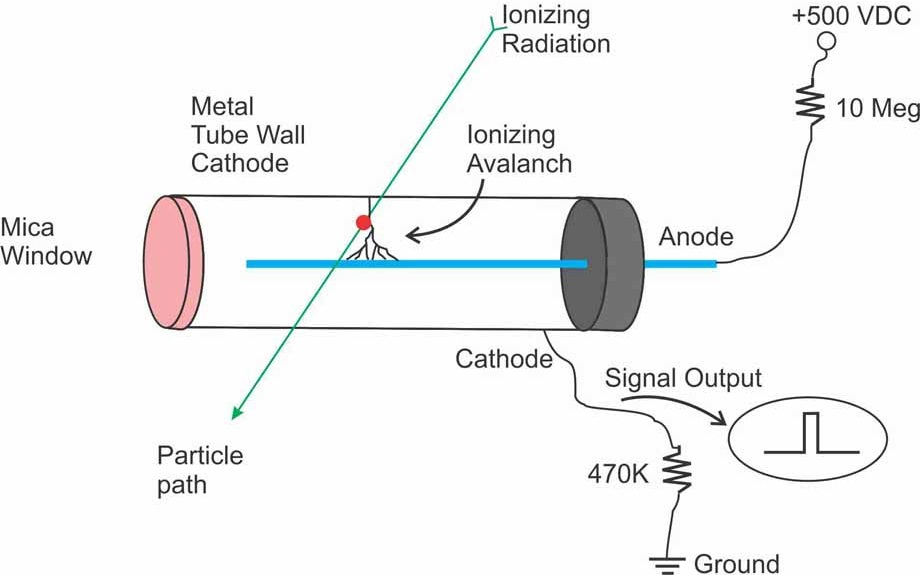
\includegraphics[width=1\columnwidth]{images/th.jpg}
    \caption{Schematic setup of a GM Counter}
    \label{t1}
\end{figure}

As shown in Fig. \ref{t2} the operating voltage of the GM counter is set in the plateau region, where the counting rate is relatively constant. The plateau length and slope determine the stability of the counting rate, while the dead time, resolving time, and recovery time limit the counting rate. The GM counter is insensitive to ionizing events during the dead time, and the resolving time and recovery time set the minimum time interval between two distinct and normal-size pulses, respectively. Higher voltages and the gas composition inside the GM tube can reduce the effects of these factors. The background counting rate can be due to cosmic rays, electronic noise or other active sources in the same room.

\begin{figure}
    \centering
    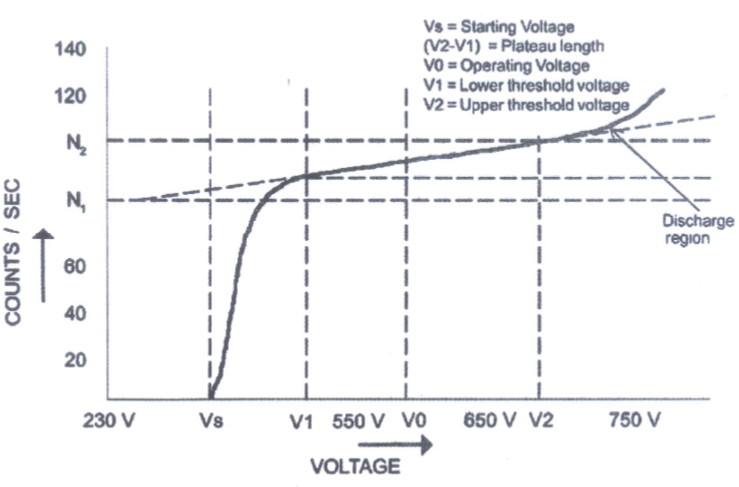
\includegraphics[width=1\columnwidth]{images/t2.png}
    \caption{Typical voltage characteristics of a GM Counter}
    \label{t2}
\end{figure}

\subsection{Inverse Square Law}
It states that the gamma radiations reduce inversely proportional to the distance, $d$, between the detector and the radiation source. Thus, the counting rate, $R$ (counts/second), should be related as follows,
\begin{align} \label{inv-eq}
    R &\propto \frac{1}{D^2} \nonumber\\
    \therefore \log(R) &= -2\times\log(D) + C
\end{align}
\noindent where C is some constant.

\subsection{Efficiency of GM counter}
If the current activity of a radioactive source is denoted as $A$, the fraction of emitted gamma radiation that enters the GM tube is given by:

\begin{align}
    R = A \times \frac{\pi d^2/4}{4 \pi D^2} = A \times \frac{d^2}{16D^2}
\end{align}

where $D$ is the distance from source to the end window and $d$ is the diameter of the end window. 
The activity of a radioactive substance follows the
exponential decay law:
\begin{align}
    A = A_0 e^{-\lambda t}
\end{align}

where $A_0$ represents the initial activity, $\lambda$ is the decay constant, and $t$ is the elapsed time. 

\begin{align} \label{half}
    \lambda = \frac{\ln(2)}{T_\text{half}}
\end{align}

The efficiency (E) of a GM detector for gamma radiation is defined as the ratio of the counts per second (CPS) to the disintegrations per second (DPS), which is expressed as:

\begin{align} \label{eff}
    E = \frac{\text{CPS}}{\text{DPS}} = \frac{N}{R}
\end{align}
\subsection{Counting Statistics}

Say $N_i$ denote the $i^{th}$ reading of a measurement in a set of $n$ measurements, then the equations for calculating mean ($\bar{N}$), variance $\sigma^2$, and standard deviation $\sigma$ (for large samples, as dictated by the law of large numbers) are:

\begin{align}\bar{N} &= \frac{1}{N}\sum_{i = 1}^{n} N_i\\
\sigma^2 &= \frac{1}{n} \sum_{i = 1}^{n} (\bar{N} - N_i)\end{align}
% ========================================================================
\section{Experimental Setup}

\subsection*{Apparatus}

\begin{enumerate}
    \item Cesium-137 (Gamma Source)
    \item Thalium-204 (Beta Source)
    \item GM counting System
    \item GM detector
    \item Sliding Bench
    \item Detector Stand
    \item BNC cable
\end{enumerate}

\begin{figure}
    \centering
    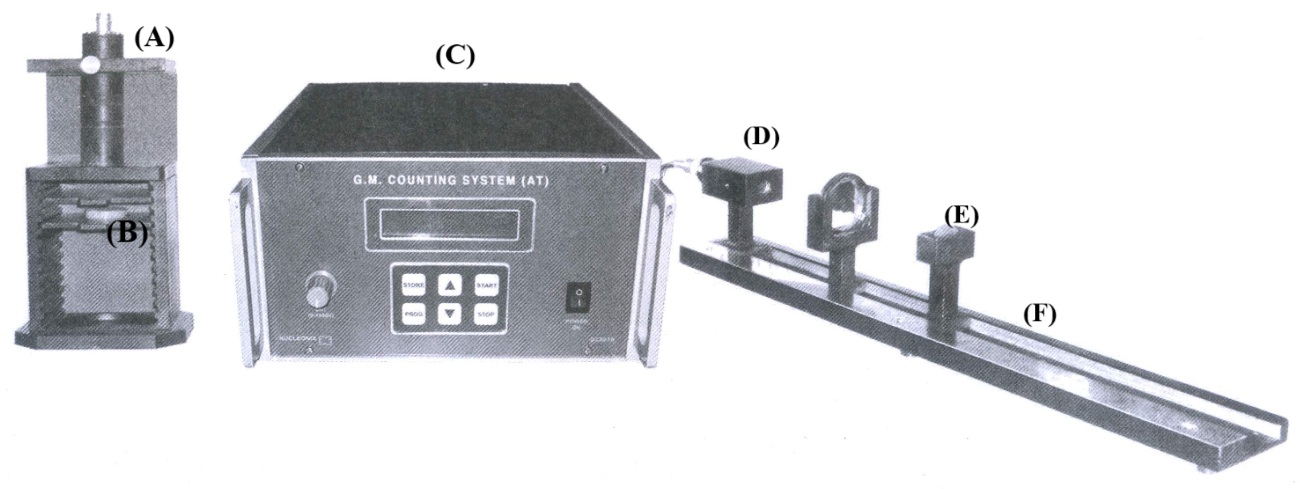
\includegraphics[width=1\columnwidth]{images/t2.jpg}
    \caption{Experimental Setup where (A) and (B) are the end window detector and source holder (C) is the GM counting system where you can vary the EHT (D) and (E) are the end window detector and source holders attached to a (E) sliding bench}
    \label{t3}
\end{figure}
\noindent Fig. \ref{t3} shows and labels all used apparatus in this experiment.